% !TeX program = xelatex
% 编译：xelatex -interaction=nonstopmode -halt-on-error Infinity高数作业报告.tex
\documentclass[UTF8,a4paper,zihao=-4,fontset=fandol]{ctexart}
\usepackage[margin=2.15cm,headheight=16pt]{geometry}
\usepackage{amsmath,amssymb,graphicx,booktabs,enumitem,xcolor,fancyhdr,hyperref}
\definecolor{inkblue}{HTML}{254E79}
\definecolor{muted}{HTML}{526273}
\hypersetup{colorlinks=true,urlcolor=inkblue,linkcolor=inkblue,pdftitle={Infinity高等数学课程作业报告},pdfauthor={Lysandra}}
\setlength{\parindent}{2em}
\setlength{\parskip}{3pt}
\linespread{1.23}
\setlist[enumerate]{leftmargin=2em,itemsep=5pt,topsep=4pt}
\ctexset{section={format=\large\bfseries\color{inkblue},beforeskip=12pt,afterskip=5pt}}
\pagestyle{fancy}
\fancyhf{}
\fancyhead[L]{\small\color{muted}Infinity · 高等数学课程作业}
\fancyhead[R]{\small\color{muted}Lysandra}
\fancyfoot[C]{\small\thepage}
\renewcommand{\headrulewidth}{0.3pt}
\begin{document}
\noindent\begin{minipage}{0.12\textwidth}
  
\includegraphics[width=1.45cm]{figures/infinity.png}
\end{minipage}\hfill
\begin{minipage}{0.85\textwidth}
  {\LARGE\bfseries\color{inkblue}Infinity：一元微积分计算应用}\par
  \vspace{5pt}
  {\small\color{muted}应用简介与开发过程\quad |\quad 开发者：Lysandra\quad |\quad 版本：2.4.1}
\end{minipage}
\vspace{8pt}
\noindent\textcolor{inkblue}{\rule{\textwidth}{0.8pt}}
\section{应用简介}
Infinity 是面向高等数学学习的一元微积分桌面应用。用户以 LaTeX 输入函数，在实时公式预览中检查表达式，再选择求导、积分或极限计算。软件以标准数学公式展示结果，并注明数值近似、适用条件或当前无法判定的情况，帮助使用者把课堂中的数学表达与计算方法联系起来。

软件使用 C++20、Qt 6 Widgets 和 CMake 开发，数学计算由本地 C++ 算法及 libqalculate 完成；KaTeX 只负责公式排版，不承担数学计算，也不依赖 Python 运行时或在线计算接口。
\begin{center}
\small
\begin{tabular}{@{}p{2.0cm}p{12.1cm}@{}}
\toprule
\textbf{功能} & \textbf{主要内容} \\
\midrule
求导 & 常见初等函数与复合函数、1--8 阶导数、指定点导数。\\
积分 & 常见原函数、正常定积分、数值积分；部分含参数表达式及条件分支。\\
极限 & 有限点、左右极限、无穷处的部分极限；区分精确值、无穷、不存在与无法判定。\\
辅助工具 & 多函数绘图、选点切线与方程、计算历史、多项式化简及数值算法实验。\\
\bottomrule
\end{tabular}
\end{center}
\begin{center}
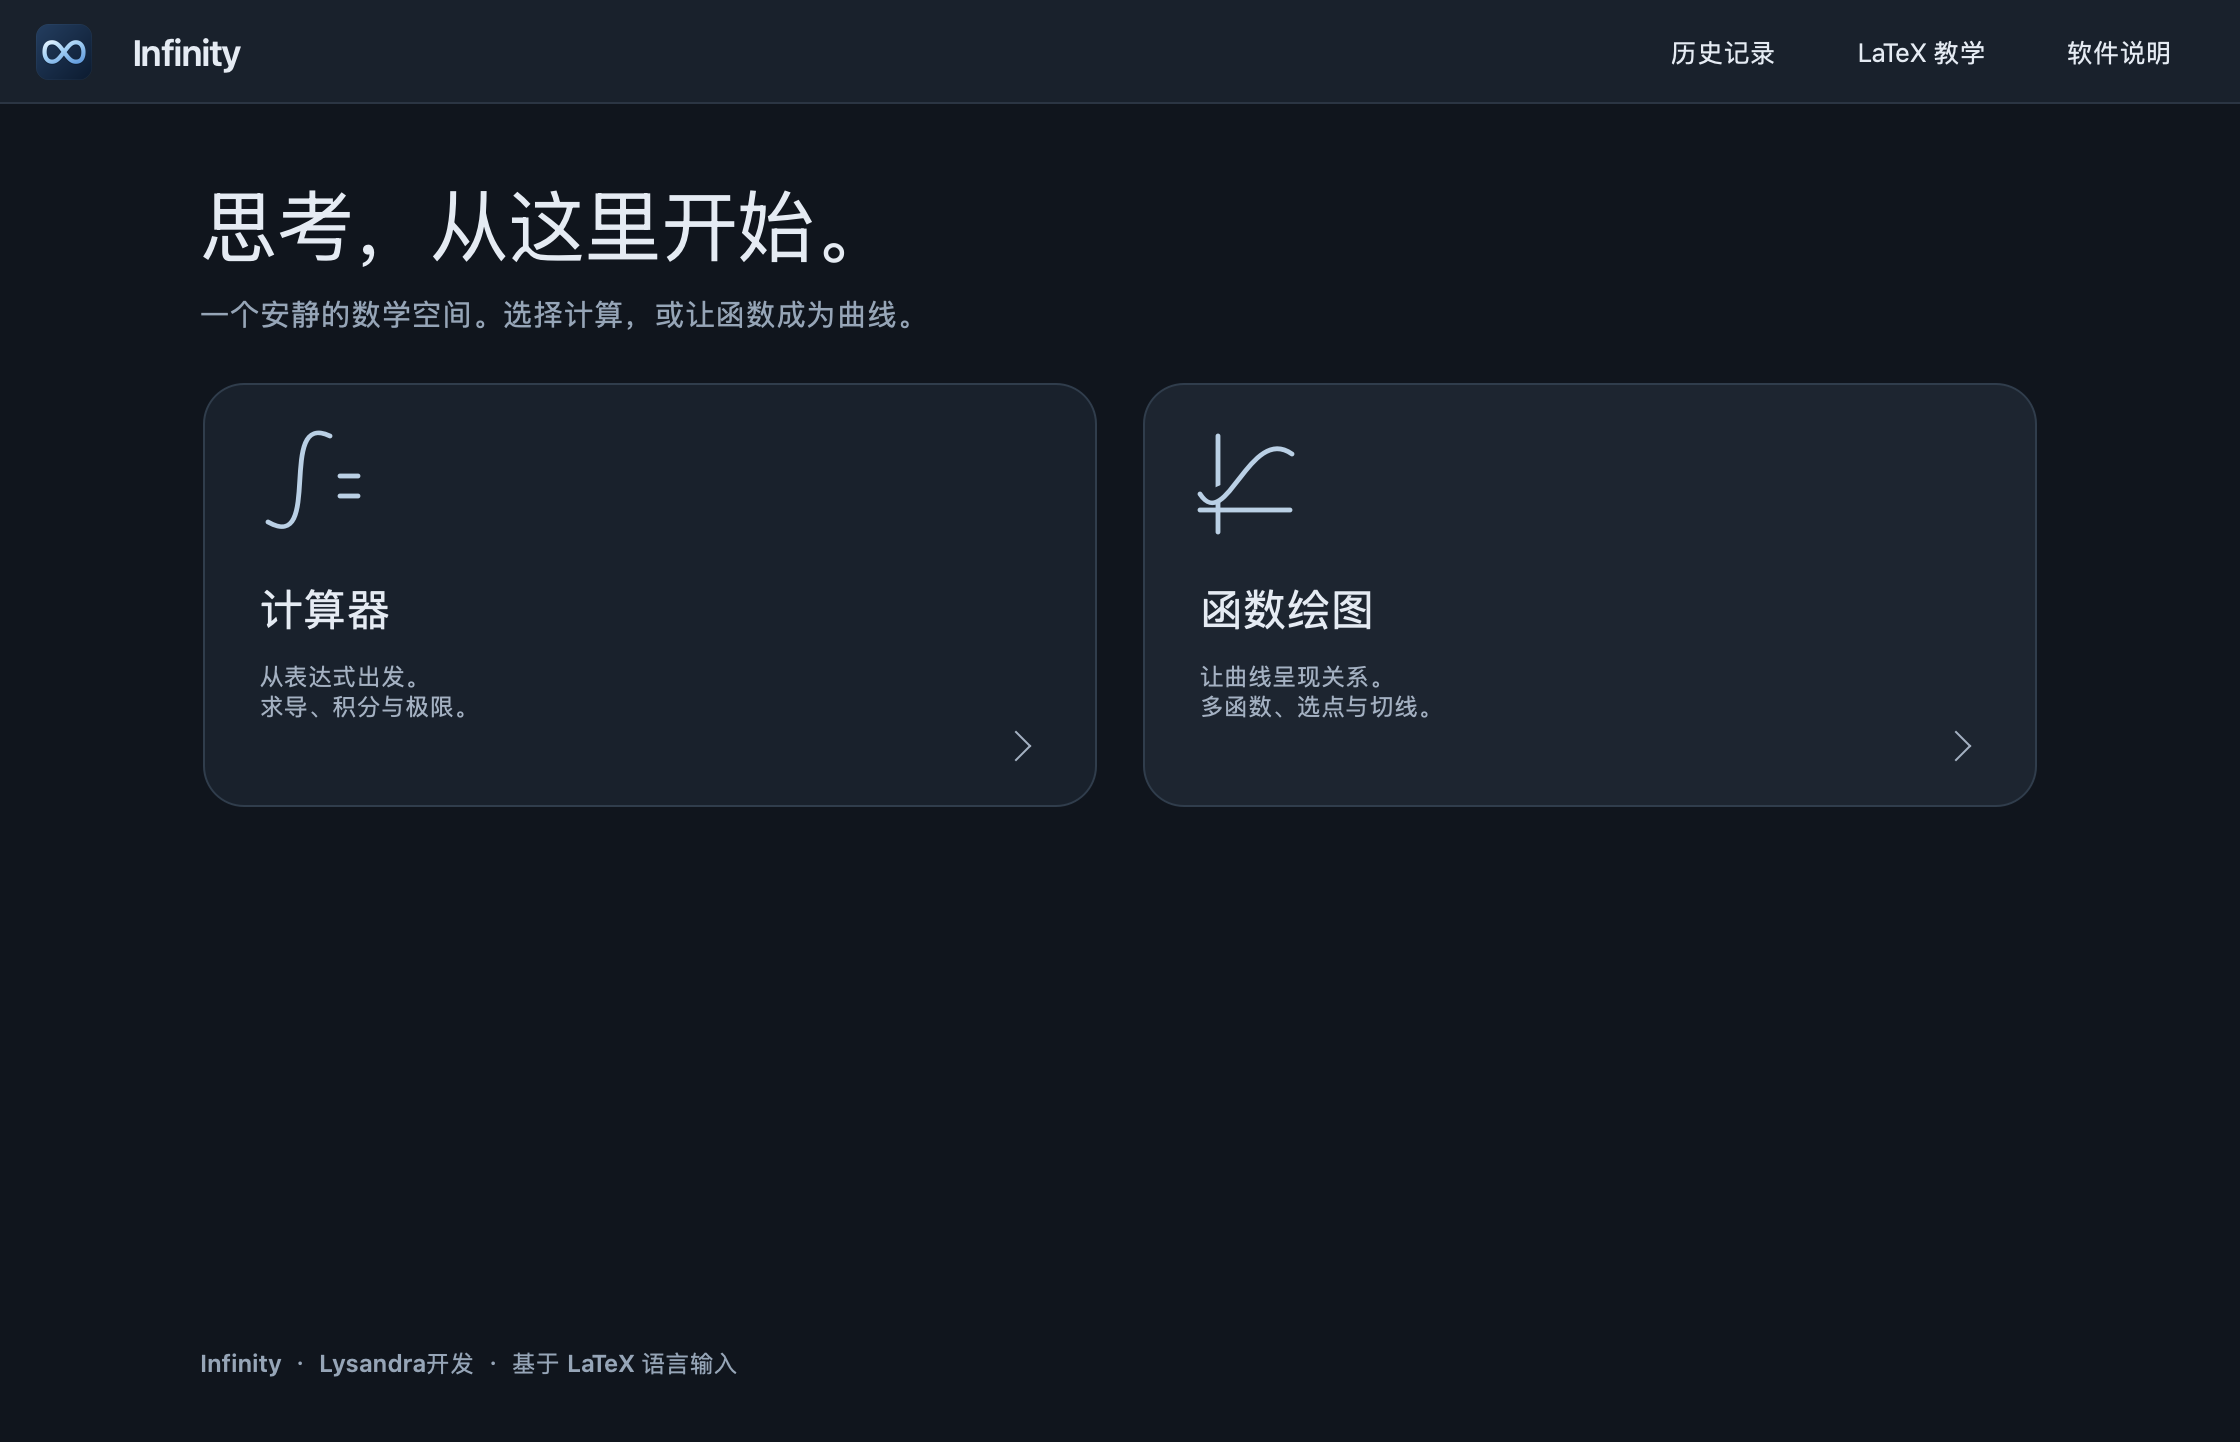
\includegraphics[width=0.81\textwidth]{figures/home.png}\par
\vspace{2pt}
{\small\color{muted}图 1\quad 应用首页：计算器与函数绘图双入口，公式采用 LaTeX 输入。}
\end{center}
\newpage
\section{开发过程}
\begin{enumerate}
\item \textbf{建立可运行的工程。}采用 CMake 管理 C++ 工程，将界面、表达式解析、符号计算、数值算法和绘图分离。先完成输入、求值、绘图与测试的最小版本，再逐步增加微积分能力。
\item \textbf{实现安全的公式输入。}通过分词和递归下降解析，将 LaTeX 表达式生成抽象语法树（AST）。解析器只接受白名单内的运算和函数，对错误括号、未知命令等给出提示；公式排版与数学解析分别实现。
\item \textbf{扩展数学计算。}求导使用表达式树的乘积、商与链式法则；积分结合符号库、换元和根式有理化等有限规则，并尽可能通过求导检查原函数；极限结合连续性、解析展开、阶数比较与夹逼规则，不把数值采样当作存在性证明。
\item \textbf{完善交互与参数处理。}将界面调整为简洁的蓝色首页与计算页面，增加历史窗口、公式复制、教学入口和图像导出。参数 $a,b,c,n$ 默认是实数，结果中直接显示非零条件、定义域及已支持的退化分支。
\item \textbf{测试与修正。}通过自动化测试覆盖算法和输入边界，并实际启动应用检查公式排版、导航与切线交互。检查中修复了夹逼规则忽略定义域、外层运算掩盖内部无定义值等问题，并对仅经过数值抽查的原函数明确标注验证程度。
\end{enumerate}
\section{数学方法与实验示例}
对于高阶无穷小抵消，利用
$e^x=1+x+\frac{x^2}{2}+O(x^3)$，比较首个非零项可得
\[
\lim_{x\to0}\frac{e^x-1-x}{x^2}=\frac12.
\]
对于带实数参数的积分，需要保留例外情况。在 $x>0$ 上，软件按分支返回
\[
\int x^a\,\mathrm{d}x=
\begin{cases}
\dfrac{x^{a+1}}{a+1}+C,&a\ne-1,\\[3pt]
\ln x+C,&a=-1.
\end{cases}
\]
这说明符号计算除了输出公式，还必须处理参数条件和实数定义域。对候选原函数求导，可以检查其是否还原为原来的被积函数；有限点抽查则只能发现部分错误，不能替代恒等证明。
\section{完成情况与局限}
最近一次完整回归记录为 \textbf{18 项测试全部通过}，其中包含新增的 15 项定义域断言；桌面测试覆盖 34 条计算或错误拒绝流程。macOS Apple Silicon 版本已完成本地编译、运行与独立应用包验证；Windows 保留跨平台源码与打包流程，尚未在 Windows 环境完成构建和验收。

目前不能保证求解整本教材的所有题型。反常积分、全部参数分支及符号积分边界仍未完整支持，部分原函数只经过数值抽查，绘图也可能漏掉极窄间断。后续将优先完善条件推理、符号边界输入和跨平台验收，使数学正确性与使用体验同步提高。
\end{document}
